\section{Methodology}
\label{sec:methodology}

\subsection{Attack Overview}
As discussed in the threat model, given a target application implementing a query on a given DSP system, the attacker
knows the data schema and the structure of the query DAG. Its goal is to recover the DAG content, that is, the
identities of the DAG operators. The attacker achieves this in two phases, as depicted in Figure~\ref{fig:attack-flow}:
the offline phase and the online phase.

\subsubsection*{Offline phase}
In the offline phase, the attacker profiles individual operators that are {\em similar} to the target operators, using
{\em synthetic data}. The goal is to learn to distinguish different operators based on their execution
time. This is based on the insight that in a vanilla implementation of the DSP system, operators have different
timing (or latency) distributions. For example, a stateless operator such as map and filter will have lower latency than
a stateful operator like join. The variance in the timing distribution will also be lower for stateless operators than
for stateful ones.

The attacker first instantiates the stream processing engine with a single operator running inside an enclave. This
environment approximates the real, target environment, even though the attacker does not know which operator is running
in the target application. As discussed in our system model (Section~\ref{sec:model-system}), the attacker knows the
source code of the DSP system and the enclave code of the Job Manager and Task Manager. It then runs the system with
one Job Manager enclave and one Task Manager enclave. It constructs a Job Graph consisting of one operator of its
choice and sends it to the Job Manager enclave. The only difference between this environment and the real one is the Job
Graph containing the specification of the operator (i.e., which operator and which parameters). In the attacker-controlled environment, the attacker can specify any operator with any parameters of their choice.  

Next, the attacker creates synthetic datasets based on the known schema and the operator being profiled. In particular,
starting with the original schema, it generates smaller schemas containing subsets of the original fields and synthesizes data records with random values (of the correct field types). The diverse datasets ensure that the attacker
can capture timing profiles of the target operator under varying conditions. The attacker sends the encrypted,
synthesized data records to the system and records fine-grained execution time at the Task Manager enclave. The result is a set of time series traces per operator, where each data point in a trace corresponds to the time it takes
for the operator to process one data record.   

The execution traces form the dataset for training a two-stage machine learning model. In the first stage, a classifier
is trained to identify the type of operator based on the timing data. In the second stage, a set of regression models is
trained to infer the parameters of each operator. We focus on predicting two common parameters: the window size and the
sliding step used in windowed operators.

\subsubsection*{Online phase} 
In the online phase, the attacker runs the target application and passively collects timing data for each target operator. Even when the target query DAG comprises multiple operators, our threat model (Section~\ref{sec:model-threat}) allows the attacker to execute each operator in isolation, i.e., in an isolated Task Manager enclave. The measurement is done in the same way as in the offline phase. Given the collected data, the attacker uses the previously trained models to perform inference. First, it uses the classifier to identify which operator is running. Next, it uses the corresponding regression model to predict the operator's parameter values. Through this process, the attacker recovers the full query
DAG, thereby gaining insight into proprietary application logic.



\subsection{Attack Implementation}
\subsubsection*{DSP system}
We implement a simplified version of the DSP system to demonstrate our attack. Our implementation retains the same
execution semantics as that of a full-fledged, production-ready DSP system. The system is implemented in C++ using
Intel’s SGX SDK~\cite{sgxsdk}, and each query operator runs in isolation
within its own enclave. It uses {\em hot call}\cite{hotcall}, instead of the traditional ecall/ocall or switchless
call~\cite{switchlesscall}, as the primary I/O interface between the untrusted and trusted parts of the application. The
hot calls lead to significant performance improvement compared to the alternative I/O interfaces.  They also reduce the
enclave's exposure to known communication-based vulnerabilities. Figure~\ref{fig:architecture-overview} shows the
overview of the implementation and how the attacker measures the execution timing.

\begin{figure}
    \centering
    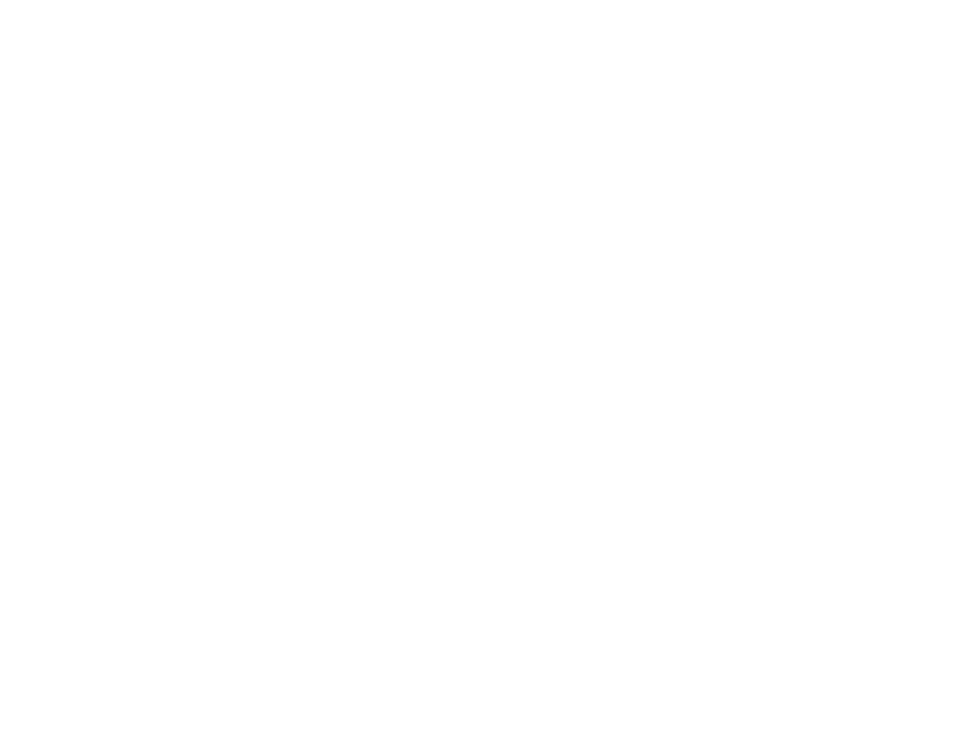
\includegraphics[width=0.49\textwidth]{Figures/engine_architecure.pdf}
    \caption{Overview of the DSP implementation and timing measurement against the enclave running a query operator.}
\label{fig:architecture-overview}
\end{figure}

Our implementation consists of two components: an untrusted part, which manages data I/O and coordinates operator
chaining, and a trusted part running inside an enclave and executing the operator's computation logic.  It is
multi-threaded, with concurrent threads operating in a pipelined fashion. The data records are processed in five steps as follows. 

First,  the source thread, running outside the enclave, reads the encrypted data from external sources (e.g., files or network streams). It pushes the records into an in-shared buffer, which is in a memory region shared between the untrusted part and the enclave. Second, inside the enclave, an event receiver thread continuously polls the in-shared buffer for new data. When a new
data record is detected, it is pulled into the enclave using a hot call, then decrypted. Third, the decrypted data is passed to the operator, which performs the intended computation (e.g., filter, map, join, aggregate) and produces an intermediate result. Fourth, the result is sent to an event sender component within the enclave, which encrypts and pushes it into the
out-shared buffer, another shared memory region between the enclave and the untrusted part. Fifth, in the untrusted part, a sink thread (running concurrently with the source thread) continuously polls the
out-shared buffer. It fetches the encrypted results when available, then either forwards them to the next enclave in the
processing pipeline or stores them in persistent storage, such as a database or CSV file.

%By isolating each operator in its own enclave and leveraging a
%modular, multithreaded design, our system enables precise, per-operator timing measurements, making it a suitable
%platform for evaluating microarchitectural side-channel risks in stream processing workloads.

\subsubsection*{Shared buffers}
The shared buffers in our system are implemented as circular buffers, a data structure commonly used in multi-threaded
environments to support ordered communication between producers and consumers. A circular buffer uses a fixed-size array
in a way that treats the beginning and end as contiguous, enabling continuous data flow without moving the elements.

% \begin{figure}[htb]
%     \centering
%     \includegraphics[width=0.49\textwidth]{Figures/circular-buffer.pdf}
%     \caption{Circular Buffer}
%     \label{fig:circular-buffer}
% \end{figure}

Each buffer maintains two pointers: a head pointer (also known as the write pointer), pointing to the position where
the next incoming data item will be written, and a tail pointer (or read pointer), pointing to the position where the
next data item will be read. When the producer writes data and the buffer is not full, the head advances to the next
slot in the array, inserting the new element. Conversely, when the consumer reads data, the element at the tail is
retrieved, and the tail pointer advances to the next unread item. If either pointer reaches the end of the array, it
wraps around to the beginning, enabling circular traversal of the buffer. This wrapping behavior makes it suitable for
streaming scenarios, especially under memory constraints. When the head and tail pointers collide, the buffer is
considered full, and further writes are blocked until space is freed.

In our implementation, each circular buffer is encapsulated as an object, exposing a \textit{push()} method used by source threads or enclaves to insert new data records, and a \textit{pop()} method used by enclaves or sink threads to retrieve available data.
The buffers enable thread-safe communication between the untrusted and trusted components of the system.

\subsubsection*{Data encryption and decryption}
All data in both in-shared and out-shared buffers is encrypted. They are decrypted only when inside the enclaves. We use the AES-GCM 128-bit scheme for encryption and decryption operations. AES-GCM  guarantees both data integrity and confidentiality. The SGX SDK provides out-of-the-box the implementation of AES-GCM, which is accessible through two functions: \textit{sgx{\_}aes{\_}gcm{\_}encrypt} and
\textit{sgx{\_}aes{\_}gcm{\_}decrypt}. In the untrusted part, we use the OpenSSL \cite{openssl} implementation of AES-GCM. For simplicity, we hardcoded a fixed key inside the enclave's source code.

%When performing the encryptions and decryptions AES scheme, the two most important information are the key and the
%nonce. For the key's value, it is assumed that the key can be exchanged between the outside and the engine inside the
%enclave through remote attestation. Therefore, this work uses a fixed value of key and hard-coded it inside the
%enclave's source code. For the nonce's value, a new "random" value will be generated each time an encryption is
%performed.

\subsubsection*{Query operators}
Each operator is implemented as a function that takes one or two (e.g., for join operators) data records as input, performs
some computation, and then returns the result. The operator can be stateful, i.e., maintaining some intermediate states
between inputs. The functions operate on decrypted data: the input is decrypted inside the enclave before being passed
to the function, and the output is encrypted before being written to the out-shared buffer.
%is responsible for processing data only, while the encryption \& decryption
%operations and transferring data between untrusted \& trusted parts are handled by the engine.  Detailed implementation
%of each operator will be presented in the Evaluation section.
{For window operators, we implement \textit{sliding window}, in which window and sliding step sizes are based on event counts.}


\subsection{Timing Measurement}
% \begin{figure*}[htb]
%     \centering
%     \includegraphics[width=0.8\textwidth]{Figures/observer-mechanism.pdf}
%     \caption{Observer Mechanism}
%     \label{fig:observer-mechanism}
% \end{figure*}

We use the RDTSCP instruction, a variant of the RDTSC instruction, to measure the execution time of each operator in clock
cycles. On production SGX systems, RDTSC and its variants are not allowed inside the enclave, therefore we make all RDTSCP calls in the untrusted part. When using RDTSCP to measure the cycle count of a user-space operation, it 
is important to ensure that there are no context switches to the operating system, which would contaminate the
measurement. To minimize these switches, all CPU cores allocated for the enclave execution are isolated such that no
other applications are running on them.  In addition,
instead of the default scheduling algorithm of the operating system, we leverage CPU affinity to bind each thread to a
specific CPU core to minimize interference. The system runs on a data stream consisting of millions of events over a long
period of time, which helps reduce the impact of noise and other sources of timing contamination.

%When running a pipeline that contains a number of operators, the engine does not bring the whole pipeline into a single
%enclave. Instead, each operator will be allocated to and operating in its own enclave, and the measurements will be
%performed for each enclave independently. With that running strategy, each enclave is basically an operator ingesting
%data events from its in-shared buffer and producing the result to the out-shared buffer, which actually is the in-shared
%buffer of the next enclave/operator.

The attacker cannot measure processing time from inside the enclave, due to the assumption that the hardware is secure.
Therefore, all timing measurements must be done from outside the enclave, i.e., in the untrusted part. As shown in
Figure~\ref{fig:architecture-overview}, for each enclave, the measurement is performed by the Observer
thread, which continuously observes the changes in the in-shared buffer of the enclave and records the RDTSC value each
time a change is detected. Particularly, the Observer thread repeatedly checks the value of the tail pointer of the
observed buffer. If the current value of the tail pointer is different from the last recorded value, that means the
enclave has ingested a new data event for processing.  The Observer thread will record RDTSC at that moment immediately,
and the tail pointer's current value will be saved as the most recent value. Finally, the processing time for a data
record is computed by subtracting the previous recorded RDTSC value from the newly recorded one. By experimenting with
each operator with a large number of data records, the attacker can obtain a large number of processing times, which form the
dataset for training machine learning models that predict the operator logics and parameters.

\subsection{Machine Learning Model Settings}
We perform a number of pre-processing steps on the data collected from running the operators with synthetic data. These steps prepare the data for training the machine learning models. Specifically, for each time series, we discard the first and last 5\% of data points.  We remove these segments because they are noisy due to the system warming up and termination.  The remaining 90\% of the time series, capturing the steady-state data, is then transformed into fixed-length representations. 
%
This is necessary because the time series have varying lengths and therefore cannot be directly input into standard classifiers. We employ two transformation methods. The first is a statistical method based on the \textit{cumulative distribution function (CDF)} of the time series. The second is a representation learning method using \textit{TS2Vec}~\cite{yue2022ts2vec}, a self-supervised embedding model that generates compact representations of the time series. 
%These two approaches yield fixed-length feature vectors that are used as input for the learning models.


{\bf CDF-based representation.} The reason for using CDFs is that they capture the empirical distribution of data points in a compact representation,  while abstracting away the temporal order in the time series. Given a univariate time series containing operator execution times, we generate its CDF and uniformly sample $k$ data points from the result. In our implementation, we empirically set $k=1024$, obtaining a fixed-size vector of 1024 values representing the shape of the distribution.

{\bf TS2Vec-based representation.} This method transforms a variable-length time series into a fixed-length embedding vector. We use the TS2Vec model~\cite{yue2022ts2vec} that is specifically designed to capture rich temporal features and dynamics in time series data. TS2Vec works by training a self-supervised model. Due to limited resources, we trained the TS2Vec model for only 10 epochs, with the output embedding dimension set to 1024 --- the same dimensionality in the CDF-based method to enable a fair comparison. Specifically, we trained TS2Vec on the time series collected during the offline phase, and then used the learned encoder to turn each time series into an embedding vector for downstream classification and regression tasks.

{\bf Models.} We select three simple, lightweight machine learning models, namely Random Forest, Support Vector Machine (SVM), and XGBoost. These models demonstrate accuracy while remaining efficient and are amenable to model interpretability.  
%More complex models, such as deep learning-based approaches, are left as future work.
